\section{Corpus geometry and source weighting}
\label{app:corpus}
\begin{table}[tb]
\centering\small
\caption{Geometry and source concentration of the principal E1 cohorts. Mean and median describe prepared clip duration. No context means the at-most-two-second target covers the clip. Added is the mean total observed context across both sides under the frozen placement rule. Max. source is the largest recording source's share of target reference units.}
\label{tab:corpus-inventory}
\resizebox{\textwidth}{!}{%
\begin{tabular}{lrlrrr}
\toprule
Corpus & Mean (s) & Median [IQR] (s) & No context (\%) & Added (s) & Max. source (\%) \\
\midrule
VLR & 5.782 & 5.64 [4.96, 6.44] & 0.2 & 0.851 & 4.8 \\
LRS2 & 1.642 & 1.44 [1.16, 1.92] & 79.3 & 0.099 & 3.2 \\
Spanish & 5.913 & 4.30 [2.16, 7.79] & 23.2 & 0.596 & 24.9 \\
ViCocktail & 5.830 & 5.16 [4.24, 7.00] & 0.9 & 0.843 & 13.4 \\
\bottomrule
\end{tabular}%
}
\end{table}

\begin{table}[tb]
\centering\small
\caption{Ranges after omitting one recording source at a time from the principal selected-system comparison. These are descriptive source-influence ranges, not confidence intervals. The primary source-bootstrap uncertainty remains in Table~\ref{tab:primary-intervals}.}
\label{tab:source-influence}
\begin{tabular}{lll}
\toprule
Corpus & C--A range (pp) & C--B range (pp) \\
\midrule
VLR & [-8.278, -7.990] & [-0.152, -0.139] \\
LRS2 & [-2.421, -2.226] & [-1.962, -1.784] \\
Spanish & [-5.604, -4.969] & [-1.751, -1.111] \\
ViCocktail & [-3.919, -3.370] & [-1.210, -0.833] \\
\bottomrule
\end{tabular}
\end{table}

The duration statistics in Table~\ref{tab:corpus-inventory} describe the exact
principal assessment cohorts, measured from prepared frames at 25 fps. They
are not estimates of the complete source datasets. The interval in the median
column gives the 25th and 75th percentiles. For the two-second request, 79.3\%
of LRS2 clips already fit inside the target, compared with 0.2\% on VLR,
23.2\% on Spanish, and 0.9\% on ViCocktail. The principal hash-based start,
center and end placements further limit which margin is available. Mean
observed context is therefore smaller than the maximum 1.28 seconds across
both sides, even in corpora with substantially longer clips.

Recording sources also have different weights. The largest Spanish source
contributes 24.9\% of the target reference units, compared with 4.8\% for VLR,
3.2\% for LRS2 and 13.4\% for ViCocktail. Both principal point differences
remain favorable to projection after omitting any single source
(Table~\ref{tab:source-influence}). These descriptive ranges address the
influence of one recording; they do not imply significance or replace the
source-bootstrap intervals. In particular, the adjusted Spanish C--B
interval still includes zero. Duration, recording composition and checkpoint
history should consequently accompany any interpretation across corpora.

\subsection{Recognition by actual context availability}
\label{app:availability}
\begin{table}[tb]
\centering\footnotesize
\setlength{\tabcolsep}{4pt}
\caption{Post-hoc context-availability analysis of the frozen principal assessment,
with the same pure-CTC decoder for A/B/C. WER is in percent; C--B differences
are in percentage points with explanatory pointwise 95\% paired-source
intervals, without multiplicity adjustment. Every clip is retained.
Availability groups follow the fixed request geometry and are descriptive.}
\label{tab:context-availability}
\begin{tabular}{llrrrrl}
\toprule
Corpus & Context & Clips & A & B & C & C--B [95\% CI] \\
\midrule
VLR & None & 27 & 89.195 & 89.195 & 89.195 & +0.000 [+0.000, +0.000] \\
VLR & Left & 3,791 & 59.678 & 47.809 & 47.626 & -0.183 [-0.242, -0.124] \\
VLR & Right & 3,717 & 55.839 & 55.078 & 54.901 & -0.177 [-0.242, -0.107] \\
VLR & Both & 3,771 & 61.056 & 48.816 & 48.658 & -0.158 [-0.229, -0.087] \\
LRS2 & None & 986 & 29.836 & 29.836 & 29.836 & +0.000 [+0.000, +0.000] \\
LRS2 & Left & 83 & 33.673 & 25.510 & 24.490 & -1.020 [-1.944, -0.208] \\
LRS2 & Right & 96 & 27.014 & 23.381 & 22.275 & -1.106 [-2.070, -0.312] \\
LRS2 & Both & 78 & 34.836 & 26.230 & 24.795 & -1.434 [-2.740, -0.405] \\
Spanish & None & 217 & 84.358 & 84.358 & 84.358 & +0.000 [+0.000, +0.000] \\
Spanish & Left & 234 & 81.993 & 78.727 & 77.722 & -1.005 [-2.003, -0.472] \\
Spanish & Right & 260 & 81.271 & 80.146 & 79.351 & -0.794 [-1.366, -0.276] \\
Spanish & Both & 223 & 86.188 & 84.933 & 83.049 & -1.883 [-2.902, -1.174] \\
ViCocktail & None & 11 & 59.649 & 59.649 & 59.649 & +0.000 [+0.000, +0.000] \\
ViCocktail & Left & 361 & 54.862 & 53.120 & 52.980 & -0.139 [-0.277, -0.034] \\
ViCocktail & Right & 407 & 52.642 & 50.605 & 50.385 & -0.220 [-0.369, -0.083] \\
ViCocktail & Both & 388 & 58.996 & 54.204 & 54.089 & -0.115 [-0.382, +0.181] \\
\bottomrule
\end{tabular}
\end{table}

Table~\ref{tab:context-availability} separates the principal assessment by
whether the recorded input adds left, right, both, or no context to the target.
It uses matched pure CTC throughout. With no outside context, A/B/C return
identical predictions on all 27 VLR, 986 LRS2, 217 Spanish, and 11 ViCocktail
clips. The whole-cohort difference therefore combines an identity subset with
clips on which contextual inference can change the result.

The three LRS2 outside-context groups show C--B reductions of 1.020--1.434
points. VLR's corresponding reductions are 0.158--0.183 points, and Spanish's
are 0.794--1.883 points. ViCocktail shows smaller differences, with the interval
for its both-context group including zero. This decomposition complements the
duration experiment without excluding short clips from the principal endpoint.
The groups differ in target position and clip duration; comparisons across
groups are descriptive rather than controlled left-versus-right interventions.

\section{Primary comparison uncertainty}
\begin{table}[tb]
\centering\small
\caption{Paired source-bootstrap intervals for the eight primary system comparisons. Negative differences favor projection. Bonferroni adjustment uses 99.375\% individual percentile intervals from 10,000 draws; coverage is approximate.}
\label{tab:primary-intervals}
\begin{tabular}{lll}
\toprule
Corpus & Contrast & Difference and family-adjusted interval (pp) \\
\midrule
VLR & C--A & -8.168 [-9.086, -7.282] \\
VLR & C--B & -0.145 [-0.194, -0.097] \\
LRS2 & C--A & -2.366 [-3.377, -1.449] \\
LRS2 & C--B & -1.876 [-2.916, -0.852] \\
Spanish & C--A & -5.281 [-7.487, -3.903] \\
Spanish & C--B & -1.357 [-3.025, +0.020] \\
ViCocktail & C--A & -3.574 [-5.126, -2.001] \\
ViCocktail & C--B & -0.986 [-1.834, -0.183] \\
\bottomrule
\end{tabular}
\end{table}

Table~\ref{tab:primary-intervals} reports the complete primary family. Source
resampling preserves paired arm predictions within each sampled recording.
It addresses within-source dependence more directly than treating every
clip as independent, but it cannot account for unobserved dependence between
recordings or repair prior exposure to the assessment corpus. In particular,
the Spanish C--B interval includes zero after the family adjustment.

\section{Complete duration grids and actual context}
\label{app:duration}
\begingroup
\footnotesize
\setlength{\tabcolsep}{3pt}
\begin{longtable}{lrrrrrr}
\caption{Complete duration grids: development-selected WER (\%). Cohort sizes are VLR: 1,024; LRS2: 1,024; Spanish: 934; ViCocktail: 1,024. Target length and per-side context are maxima clipped to available video. Compare context within a fixed target; target length changes reference content. Decoders: VLR A/B/C: greedy/greedy/greedy; LRS2 A/B/C: hybrid10/hybrid50/hybrid10; Spanish A/B/C: hybrid10/hybrid50/hybrid10; ViCocktail A/B/C: hybrid10/hybrid50/hybrid10.}\label{tab:duration-grid}\\
\toprule
Corpus & Target (s) & Context (s) & Units & A & B & C \\
\midrule
\endfirsthead
\toprule
Corpus & Target (s) & Context (s) & Units & A & B & C \\
\midrule
\endhead
\midrule
\multicolumn{7}{r}{Continued on the next page}\\
\endfoot
\bottomrule
\endlastfoot
VLR & 1 & 0 & 3783 & 82.659 & 82.659 & 82.659 \\
VLR & 1 & 0.32 & 3783 & 82.659 & 60.455 & 60.005 \\
VLR & 1 & 0.64 & 3783 & 82.659 & 57.018 & 56.490 \\
VLR & 2 & 0 & 7608 & 59.727 & 59.727 & 59.727 \\
VLR & 2 & 0.32 & 7608 & 59.727 & 49.882 & 49.724 \\
VLR & 2 & 0.64 & 7608 & 59.727 & 48.686 & 48.633 \\
VLR & 3 & 0 & 11449 & 50.808 & 50.808 & 50.808 \\
VLR & 3 & 0.32 & 11449 & 50.808 & 46.161 & 46.161 \\
VLR & 3 & 0.64 & 11449 & 50.808 & 45.061 & 45.017 \\
LRS2 & 1 & 0 & 3692 & 47.481 & 47.914 & 47.481 \\
LRS2 & 1 & 0.32 & 3692 & 47.481 & 35.509 & 32.151 \\
LRS2 & 1 & 0.64 & 3692 & 47.481 & 35.049 & 29.984 \\
LRS2 & 2 & 0 & 5052 & 25.396 & 26.564 & 25.396 \\
LRS2 & 2 & 0.32 & 5052 & 25.396 & 25.238 & 23.555 \\
LRS2 & 2 & 0.64 & 5052 & 25.396 & 25.020 & 22.783 \\
LRS2 & 3 & 0 & 5353 & 22.287 & 23.445 & 22.287 \\
LRS2 & 3 & 0.32 & 5353 & 22.287 & 23.109 & 21.371 \\
LRS2 & 3 & 0.64 & 5353 & 22.287 & 22.978 & 21.409 \\
Spanish & 1 & 0 & 2423 & 105.737 & 102.889 & 105.737 \\
Spanish & 1 & 0.32 & 2423 & 105.737 & 92.035 & 92.778 \\
Spanish & 1 & 0.64 & 2423 & 105.737 & 89.889 & 87.330 \\
Spanish & 2 & 0 & 4428 & 89.499 & 89.273 & 89.499 \\
Spanish & 2 & 0.32 & 4428 & 89.499 & 86.134 & 83.424 \\
Spanish & 2 & 0.64 & 4428 & 89.499 & 83.853 & 79.991 \\
Spanish & 3 & 0 & 6143 & 79.993 & 81.605 & 79.993 \\
Spanish & 3 & 0.32 & 6143 & 79.993 & 80.905 & 78.187 \\
Spanish & 3 & 0.64 & 6143 & 79.993 & 81.345 & 77.601 \\
ViCocktail & 1 & 0 & 4483 & 70.109 & 69.708 & 70.109 \\
ViCocktail & 1 & 0.32 & 4483 & 70.109 & 62.614 & 61.923 \\
ViCocktail & 1 & 0.64 & 4483 & 70.109 & 60.228 & 59.447 \\
ViCocktail & 2 & 0 & 9019 & 54.928 & 54.862 & 54.928 \\
ViCocktail & 2 & 0.32 & 9019 & 54.928 & 51.591 & 50.815 \\
ViCocktail & 2 & 0.64 & 9019 & 54.928 & 50.194 & 48.841 \\
ViCocktail & 3 & 0 & 13733 & 49.290 & 49.712 & 49.290 \\
ViCocktail & 3 & 0.32 & 13733 & 49.290 & 46.843 & 46.137 \\
ViCocktail & 3 & 0.64 & 13733 & 49.290 & 46.232 & 45.453 \\
\end{longtable}
\endgroup

\begin{table}[tb]
\centering\small
\caption{Actual input geometry at a maximum of 0.64 s context per side. Context available counts clips with any outside video; both full counts clips with two complete margins. Input and added context are per-clip means, with added context summed across both sides.}
\label{tab:duration-geometry}
\resizebox{\textwidth}{!}{%
\begin{tabular}{lrrrrrr}
\toprule
Corpus & Target (s) & Clips & Context available & Both full & Input (s) & Added (s) \\
\midrule
VLR & 1 & 1024 & 1022 & 1021 & 2.276 & 1.277 \\
VLR & 2 & 1024 & 1022 & 1011 & 3.268 & 1.271 \\
VLR & 3 & 1024 & 1012 & 910 & 4.219 & 1.228 \\
LRS2 & 1 & 1024 & 888 & 150 & 1.526 & 0.541 \\
LRS2 & 2 & 1024 & 207 & 42 & 1.604 & 0.127 \\
LRS2 & 3 & 1024 & 53 & 13 & 1.626 & 0.035 \\
Spanish & 1 & 934 & 857 & 687 & 2.036 & 1.056 \\
Spanish & 2 & 934 & 717 & 580 & 2.712 & 0.886 \\
Spanish & 3 & 934 & 606 & 477 & 3.275 & 0.741 \\
ViCocktail & 1 & 1024 & 1022 & 1012 & 2.272 & 1.272 \\
ViCocktail & 2 & 1024 & 1013 & 1000 & 3.253 & 1.258 \\
ViCocktail & 3 & 1024 & 1002 & 753 & 4.141 & 1.162 \\
\bottomrule
\end{tabular}%
}
\end{table}

\begin{table}[tb]
\centering\small
\caption{Incremental projection effect relative to contextual direct at a maximum of 0.64 s context per side. Negative differences favor projection. Brackets are explanatory 95\% source-cluster bootstrap intervals, not multiplicity-adjusted confirmatory tests. Each contrast compares the same target and cohort.}
\label{tab:duration-projection}
\begin{tabular}{lrll}
\toprule
Corpus & Target (s) & Selected C--B (pp) & Pure CTC C--B (pp) \\
\midrule
VLR & 1 & -0.529 [-0.847, -0.222] & -0.608 [-0.996, -0.230] \\
VLR & 2 & -0.053 [-0.221, +0.108] & -0.118 [-0.281, +0.027] \\
VLR & 3 & -0.044 [-0.104, +0.017] & -0.079 [-0.156, +0.000] \\
LRS2 & 1 & -5.065 [-6.299, -3.849] & -1.408 [-1.819, -1.023] \\
LRS2 & 2 & -2.237 [-3.136, -1.368] & -0.376 [-0.583, -0.191] \\
LRS2 & 3 & -1.569 [-2.325, -0.821] & -0.112 [-0.205, -0.037] \\
Spanish & 1 & -2.559 [-4.405, -0.330] & -2.270 [-3.435, -1.430] \\
Spanish & 2 & -3.862 [-5.241, -2.146] & -1.558 [-2.205, -1.081] \\
Spanish & 3 & -3.744 [-5.054, -2.697] & -0.830 [-1.193, -0.579] \\
ViCocktail & 1 & -0.781 [-1.677, +0.035] & +0.067 [-0.153, +0.308] \\
ViCocktail & 2 & -1.353 [-2.066, -0.690] & -0.133 [-0.248, -0.012] \\
ViCocktail & 3 & -0.779 [-1.137, -0.320] & -0.102 [-0.194, -0.013] \\
\bottomrule
\end{tabular}
\end{table}

\begin{figure}[tb]
 \centering
 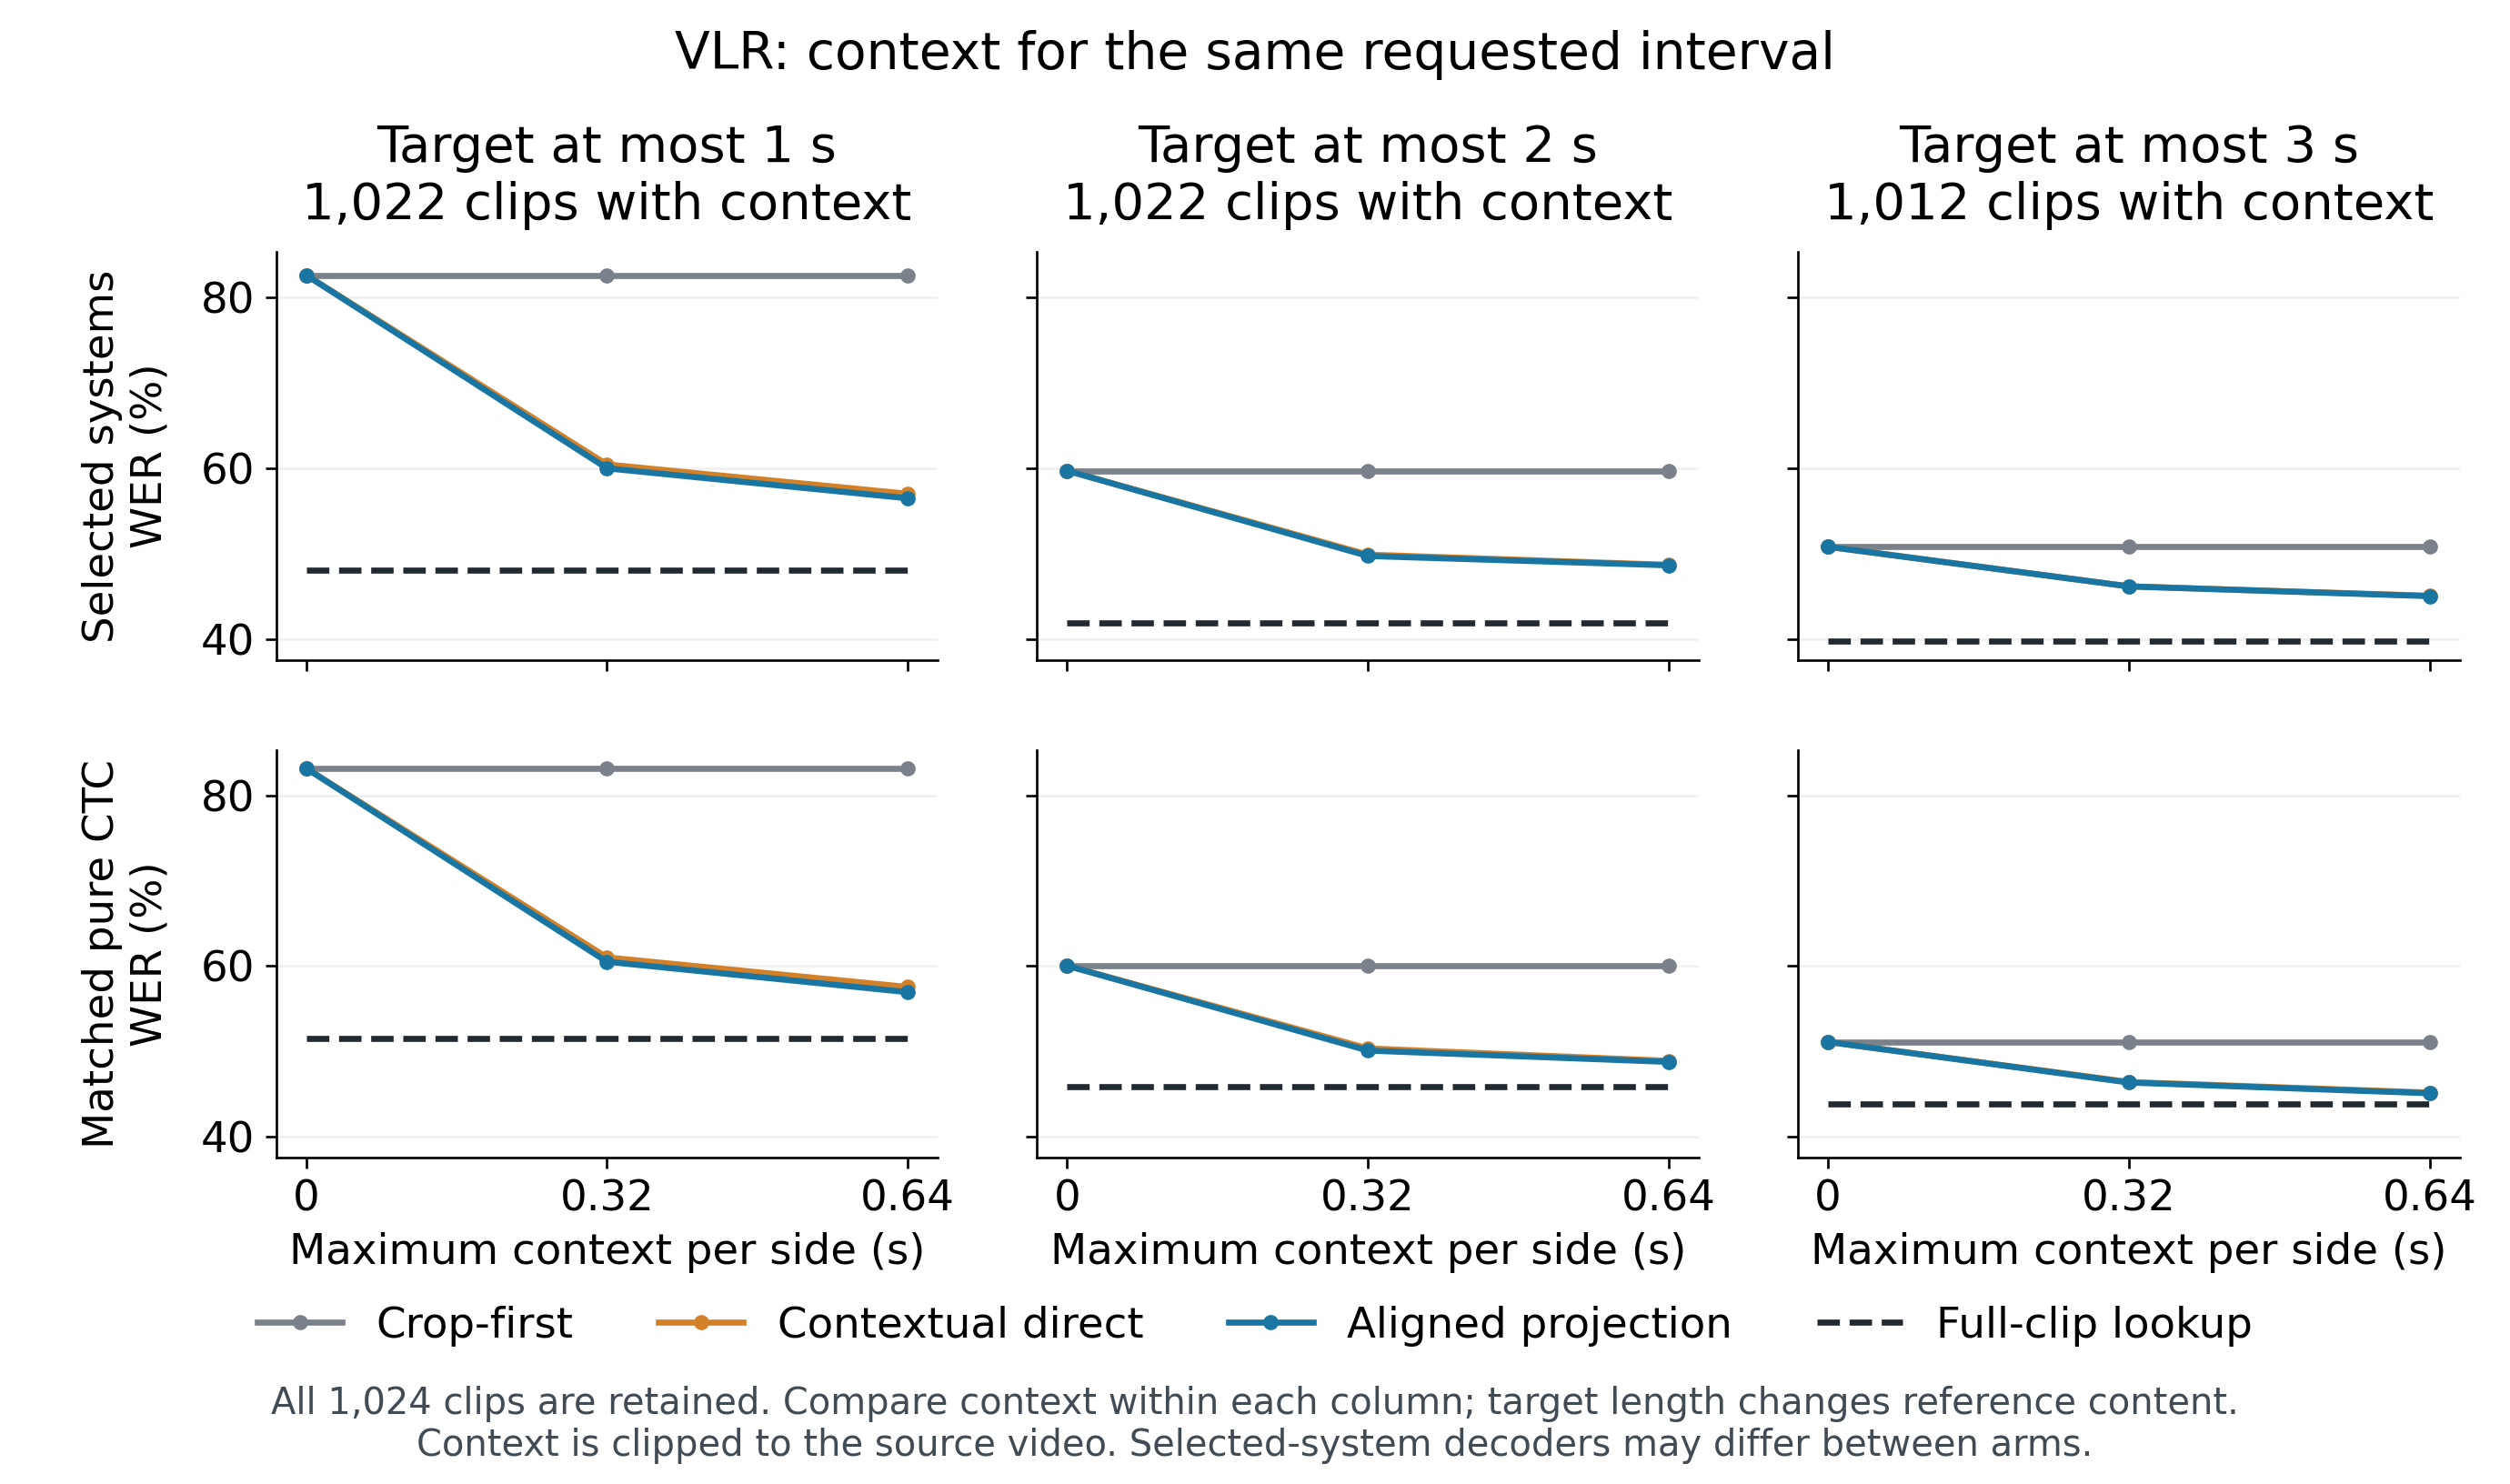
\includegraphics[width=\linewidth]{fig_VLR_T0_Context_Grid.png}
 \caption{VLR duration grid on the complete 1,024-clip cohort. Contextual
 direct and projection are close under the same greedy or pure-CTC decoder.
 The selected full-clip lookup uses a hybrid decoder, so its separation from
 the selected greedy systems includes a decoder difference.}
 \label{fig:vlr-context}
\end{figure}
\begin{figure}[tb]
 \centering
 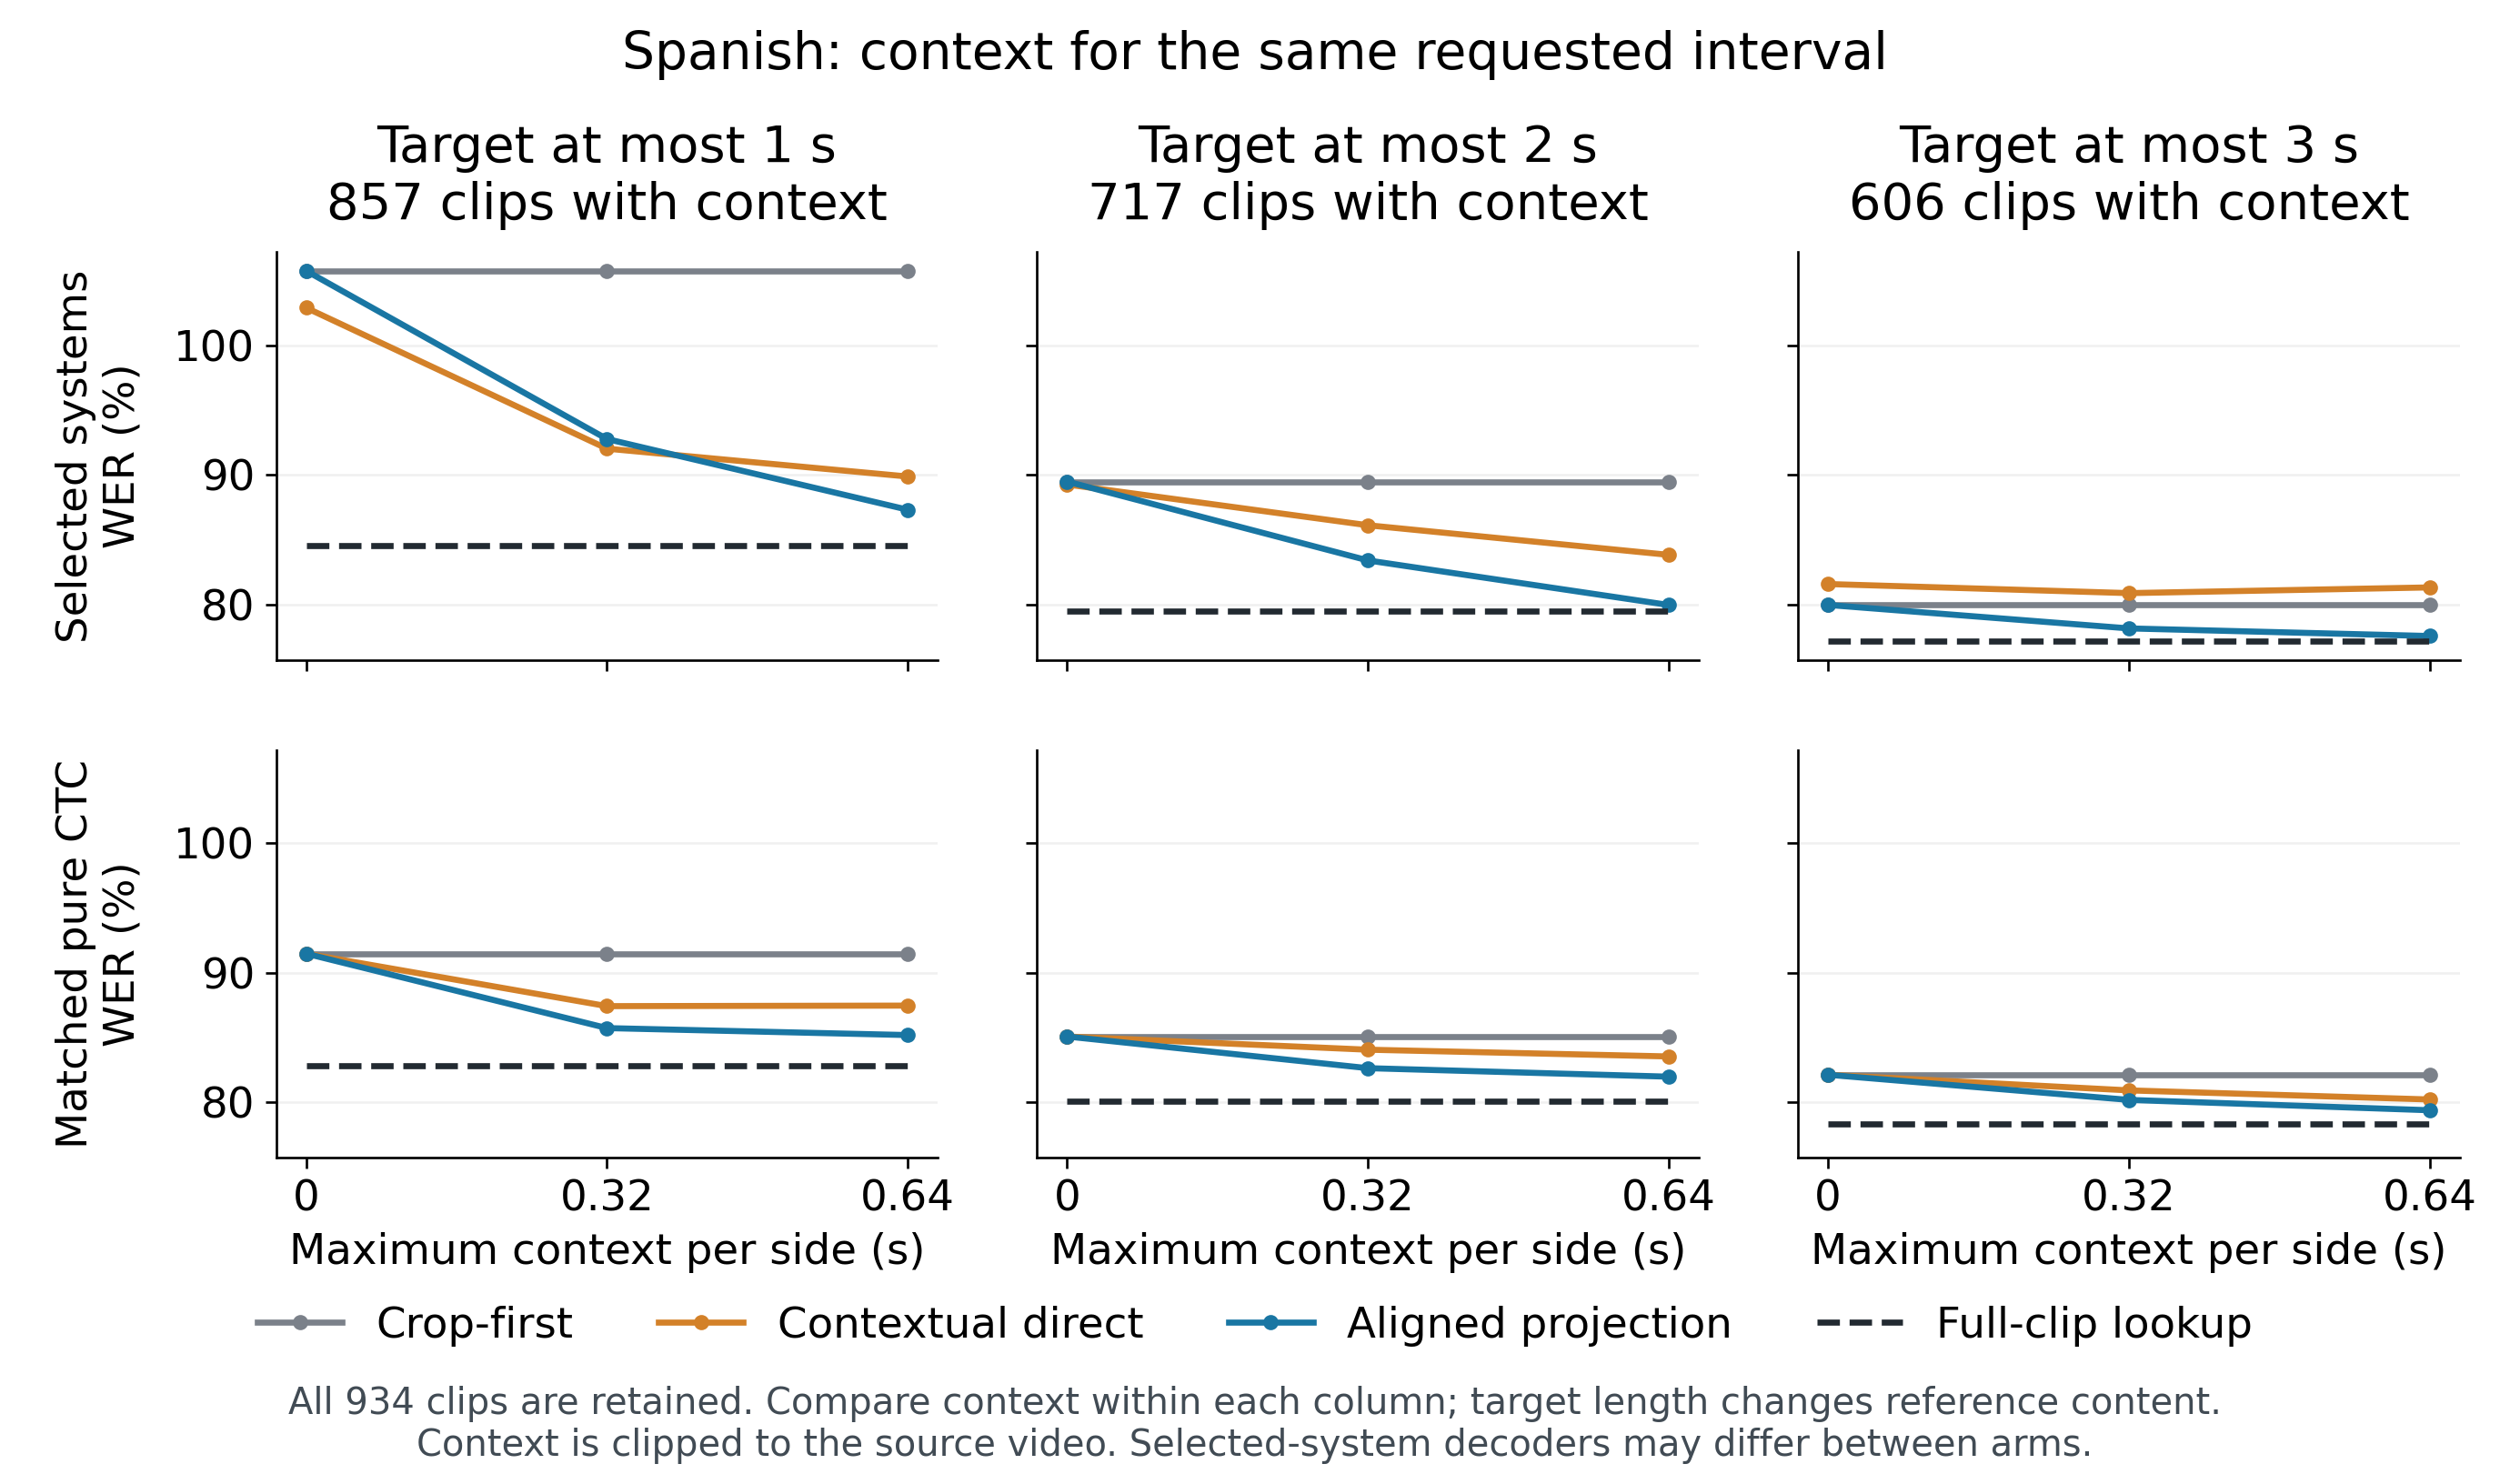
\includegraphics[width=\linewidth]{fig_ES_NATIVE_Context_Grid.png}
 \caption{Spanish duration grid on all 934 eligible clips. Native hybrid
 decoding and pure CTC have different error levels, but both support examining
 context within a fixed target. The same decoder is retained across context
 budgets within each arm. Absolute error remains high on this evaluation cohort.}
 \label{fig:spanish-context}
\end{figure}
\begin{figure}[tb]
 \centering
 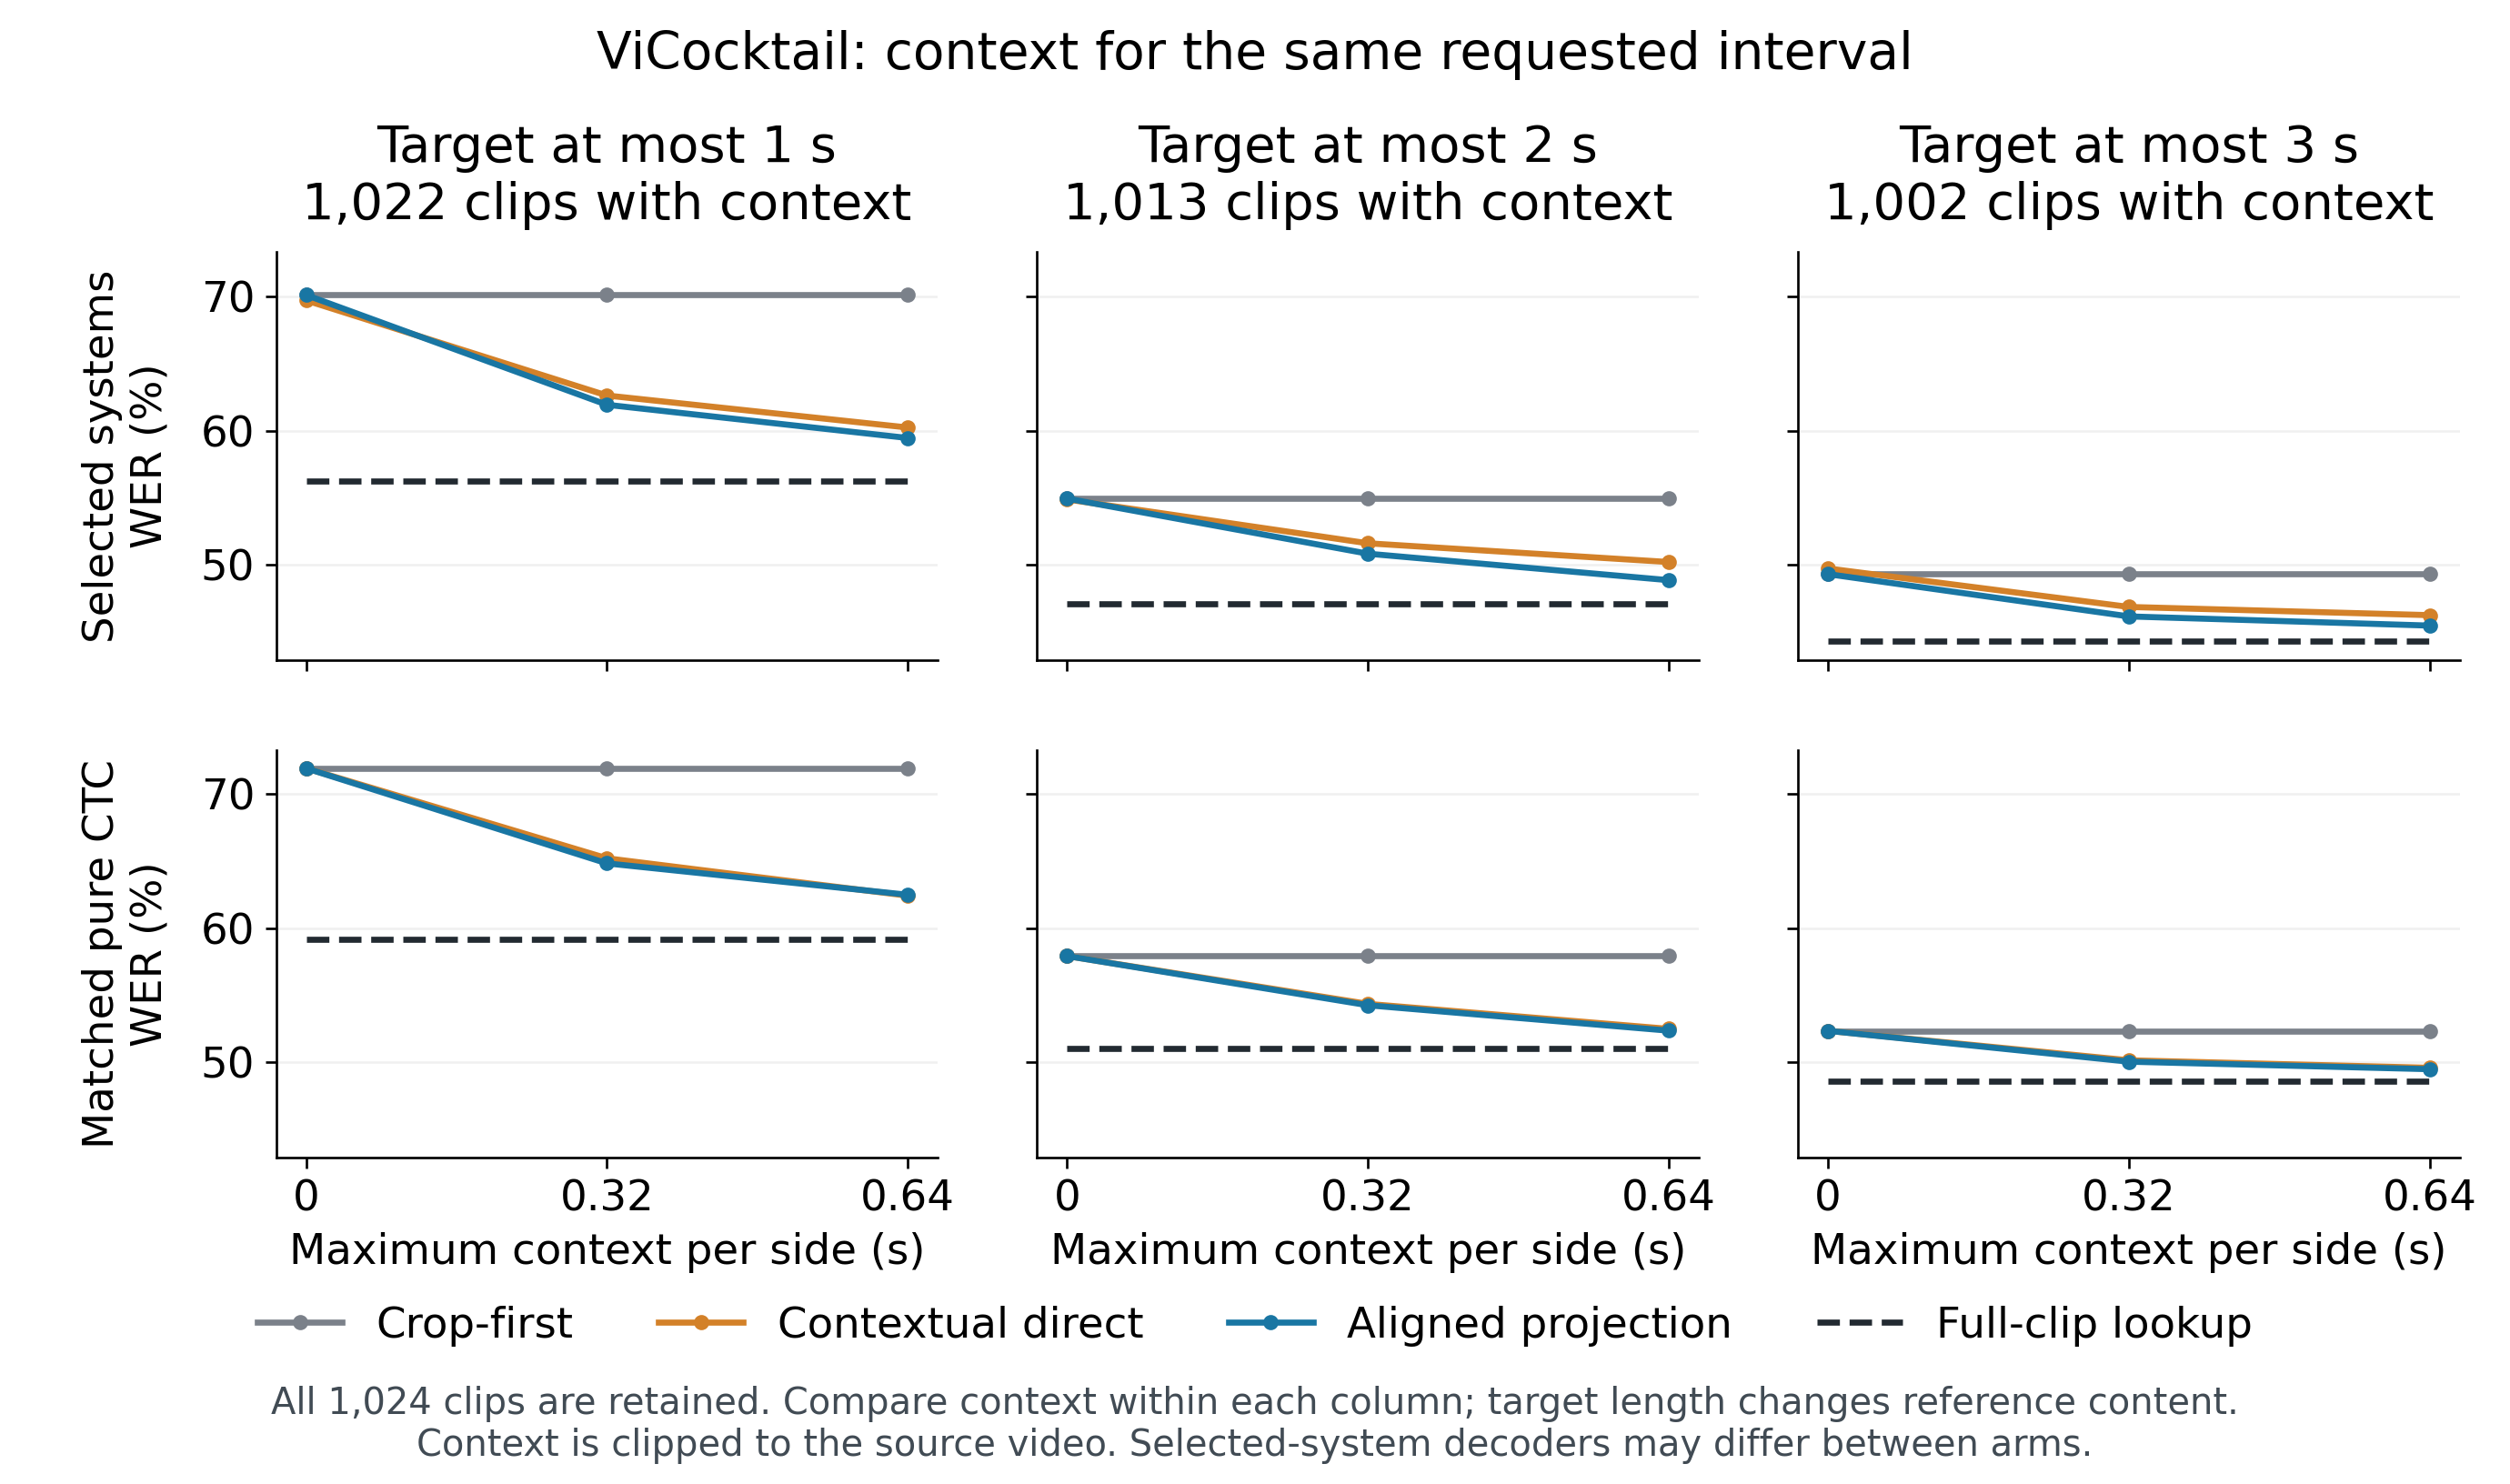
\includegraphics[width=\linewidth]{fig_VC_NATIVE_Context_Grid.png}
 \caption{ViCocktail duration grid on 1,024 clips. Context improves target
 recognition, while matched pure-CTC direct and projected readout remain close.
 The additional selected-system projection gain includes the difference
 between development-selected hybrid weights.}
 \label{fig:vicocktail-context}
\end{figure}
The nominal target and context lengths are converted to 25, 50, or 75 target
frames and 0, 8, or 16 context frames per side. All duration cells use centered
targets, while the principal two-second assessment includes deterministic
start, center, and end placements. Consequently, the duration grid is not an
exact repeat of the principal table even where the nominal lengths coincide.

At zero context, crop-first and projected output agree when the decoder is
the same. This is an identity control, not an additional recognition gain.
The full-clip target baseline is also invariant to the requested context
budget at a fixed target. Table~\ref{tab:duration-geometry} makes clipping
at video boundaries explicit. Clips without outside context remain in every
whole-cohort comparison.

Table~\ref{tab:duration-projection} keeps the incremental C--B comparisons
for every target and corpus. The Spanish matched-CTC reductions span
0.830--2.270 points, whereas the ViCocktail matched differences stay within
0.133 points of zero. The two-second Spanish C--B comparison is stronger in
this centered duration grid than in the principal placement mixture. Different
placement and cohort composition make these complementary comparisons;
the duration result does not replace the principal family-adjusted interval.
Spanish one-second selected WER can exceed 100\% because insertions contribute
to the numerator. The underlying edit counts, rather than a capped percentage,
are retained in every comparison.

\section{Complete context interventions}
\label{app:context-controls}
\begin{table}[tb]
\centering\small
\caption{Complete context interventions: requested-interval WER (\%) on the same clips with outside context within each corpus (VLR 254, LRS2 48, Spanish 202, ViCocktail 254). Targets are centered and at most two seconds. Real, repeat and reverse preserve input length; left/right retain only that margin and therefore change length. Selected A/C use greedy for VLR and hybrid10 otherwise; pure CTC is matched throughout.}
\label{tab:context-controls}
\resizebox{\textwidth}{!}{%
\begin{tabular}{llrrrrrr}
\toprule
Corpus & Regime & Crop A & Real C & Left C & Right C & Repeat C & Reverse C \\
\midrule
VLR & Selected & 60.021 & 50.211 & 51.741 & 57.806 & 54.430 & 55.538 \\
VLR & Pure CTC & 60.549 & 49.947 & 51.688 & 57.753 & 54.378 & 55.643 \\
LRS2 & Selected & 27.508 & 18.123 & 23.948 & 24.272 & 25.890 & 22.330 \\
LRS2 & Pure CTC & 33.333 & 23.625 & 28.479 & 28.479 & 31.068 & 26.861 \\
Spanish & Selected & 84.686 & 70.690 & 76.775 & 81.947 & 80.325 & 78.803 \\
Spanish & Pure CTC & 80.832 & 75.963 & 77.688 & 79.615 & 79.006 & 79.716 \\
ViCocktail & Selected & 57.116 & 50.537 & 54.876 & 54.130 & 59.823 & 60.616 \\
ViCocktail & Pure CTC & 60.429 & 54.550 & 57.210 & 57.163 & 60.616 & 61.223 \\
\bottomrule
\end{tabular}%
}
\end{table}

Table~\ref{tab:context-controls} keeps all five context conditions on the same
outside-context subset in each corpus. Both real margins give lower projected
WER than either margin alone in every displayed setting. The relative value
of the two individual margins is not constant: selected VLR projection gives
51.741\% with the left margin and 57.806\% with the right, whereas ViCocktail
gives 54.876\% and 54.130\%, respectively. Removing a margin also shortens the
encoder input and changes the native output cap, so these differences are
operating-condition comparisons rather than isolated measures of directional
linguistic information. They do not establish a language-specific rule.

Reversing each margin separately preserves its frames and length but changes
their temporal order and continuity with the target. Real context improves
the selected projected output by 5.327 points on VLR, 8.114 on Spanish and
10.079 on ViCocktail, with pointwise intervals excluding zero. LRS2 gives a
4.207-point improvement, but its interval includes zero on the smaller
48-clip subset. The matched pure-CTC contrasts have the same distinction.
Thus repeated-boundary and reversed context probe different properties;
neither intervention alone identifies the source of the recognition benefit.

For the real-versus-repeat contrast, omitting any one recording source keeps
the point difference favorable in all four corpora under both reported
decoder regimes. In Spanish, the selected-system difference ranges from
$-10.284$ to $-8.970$ points across these omissions, and the matched-CTC
difference ranges from $-3.654$ to $-2.632$. This check reduces concern that
one source alone determines the observed effect; it does not replace
evaluation on additional sources.

\section{Query-cost measurements}
\begin{table}[tb]
\centering\small
\caption{Median cumulative fresh-session response time on 32 stratified calibration clips per corpus. Three sessions are reduced to per-clip medians first. Repeated identical intervals on short clips are deduplicated. These are selected-system measurements on a GTX 1650 Ti, not matched-decoder speedups or assessment accuracy.}
\label{tab:query-cost}
\begin{tabular}{lrrrrr}
\toprule
Corpus & Requested queries & A (s) & B (s) & C (s) & F (s) \\
\midrule
VLR & 1 & 0.037 & 0.055 & 0.061 & 4.250 \\
VLR & 3 & 0.113 & 0.155 & 0.167 & 4.305 \\
VLR & 5 & 0.190 & 0.266 & 0.286 & 4.244 \\
LRS2 & 1 & 1.626 & 1.379 & 1.825 & 1.728 \\
LRS2 & 3 & 4.387 & 3.902 & 2.026 & 1.867 \\
LRS2 & 5 & 6.938 & 6.584 & 1.913 & 1.877 \\
Spanish & 1 & 1.870 & 1.623 & 3.384 & 6.212 \\
Spanish & 3 & 5.662 & 4.791 & 8.464 & 6.726 \\
Spanish & 5 & 9.256 & 7.872 & 14.321 & 6.513 \\
ViCocktail & 1 & 1.659 & 1.541 & 2.661 & 3.753 \\
ViCocktail & 3 & 4.755 & 4.465 & 6.883 & 3.740 \\
ViCocktail & 5 & 7.863 & 7.491 & 11.422 & 3.732 \\
\bottomrule
\end{tabular}
\end{table}

\begin{table}[tb]
\centering\small
\caption{Tail response cost and GPU memory under matched pure CTC. The p95 is across 32 per-clip medians of cumulative fresh-session time; memory is the median per-clip peak allocated tensor memory, including the resident model. Prepared-input loading is separate. The sample is duration-stratified, so its p95 is not a deployment-population tail estimate.}
\label{tab:matched-query-resources}
\begin{tabular}{lrrrrr}
\toprule
Corpus & Queries & C p95 (s) & F p95 (s) & C peak (MiB) & F peak (MiB) \\
\midrule
VLR & 1 & 0.71 & 1.70 & 1104.78 & 1179.58 \\
VLR & 5 & 3.45 & 1.81 & 1105.45 & 1178.28 \\
LRS2 & 1 & 0.63 & 0.82 & 1101.27 & 1101.27 \\
LRS2 & 5 & 2.75 & 0.86 & 1101.27 & 1101.27 \\
Spanish & 1 & 0.66 & 2.28 & 1105.37 & 1182.09 \\
Spanish & 5 & 3.21 & 2.41 & 1106.04 & 1180.78 \\
ViCocktail & 1 & 0.63 & 2.03 & 1098.95 & 1118.62 \\
ViCocktail & 5 & 2.99 & 2.20 & 1099.07 & 1117.32 \\
\bottomrule
\end{tabular}
\end{table}

The query schedules for one, three, and five requested intervals are separate
scenarios, not nested prefixes of one common schedule. Median cost is therefore
not required to increase monotonically between scenarios, especially after
deduplication on short clips. Full-clip lookup caches a complete recognition
and alignment result; projected inference recognizes the bounded inputs
required by the distinct requests.

Table~\ref{tab:matched-query-resources} complements the matched-decoder
median costs with the 95th percentile and peak allocated GPU memory.
These percentiles describe the stratified sample of per-clip medians;
they do not estimate a deployment-population latency distribution.
The accompanying numerical results retain duration strata, actual distinct
query counts, first and later responses, cached responses, and computation
counts. Duration strata are at most 2 seconds, (2,4], (4,8], and above
8 seconds; empty strata are omitted.

The timing endpoints include native normalization, device transfer, decoding,
and the alignment needed by the output procedure. Prepared-input reading and
decompression are measured separately. GPU memory is peak allocated tensor
memory rather than total device usage. The calibration timing experiment adds
no assessment WER measurements and cannot establish a universal break-even
number of queries.

\section{Sensitivity to reference timing}
\begin{table}[tb]
\centering\small
\caption{Ranges of point differences across seven midpoint clock settings and one overlap convention. These are sensitivity ranges, not confidence intervals. Negative differences favor C.}
\label{tab:timing-range}
\begin{tabular}{lllll}
\toprule
Corpus & Regime & C--A (pp) & C--B (pp) & C--Uniform (pp) \\
\midrule
VLR & Selected & [-12.131, -2.431] & [-0.206, -0.011] & [-8.228, +1.041] \\
VLR & Pure CTC & [-12.237, -2.571] & [-0.205, -0.029] & [-8.217, +1.095] \\
LRS2 & Selected & [-2.655, -1.766] & [-1.894, -1.728] & [-1.454, +0.245] \\
LRS2 & Pure CTC & [-2.301, -1.161] & [-0.310, -0.165] & [-1.324, +0.213] \\
Spanish & Selected & [-6.583, -2.905] & [-1.543, -0.944] & [-3.700, -0.233] \\
Spanish & Pure CTC & [-3.379, -0.615] & [-0.954, -0.462] & [-2.962, -0.212] \\
ViCocktail & Selected & [-4.071, -2.312] & [-1.176, -0.385] & [-4.235, -2.262] \\
ViCocktail & Pure CTC & [-3.631, -1.940] & [-0.159, -0.051] & [-3.748, -2.071] \\
\bottomrule
\end{tabular}
\end{table}

The seven midpoint conditions shift the reference word times by -160 ms,
-80 ms, -40 ms, 0 ms, +40 ms, +80 ms, and +160 ms while leaving target
geometry and predictions fixed. The eighth condition uses any positive temporal
overlap at zero offset.
Whole-clip targets retain their original full transcript.
These changes can alter reference membership and the denominator, so each
condition compares arms only against its own shared reference.

Table~\ref{tab:timing-range} reports the full range of differences, rather than
selecting a favorable clock shift. C--A and C--B keep negative point
differences throughout the tested conditions. C--uniform is sensitive enough
to reverse on VLR and LRS2. No clock offset or ownership convention is selected
from these assessment results.

\section{Sensitivity to decoder settings}
\label{app:decoder-sensitivity}
A separate development screen covers 256 VLR, 256 LRS2, 143 Spanish, and
256 ViCocktail clips. These clips are disjoint from the calibration clips
and from assessment sources. With the two-second target and the 0.64-second
context allowance fixed, greedy and pure-CTC decoding use blank-logit biases
of $-0.5$, $0$, and $+0.5$. Native hybrid decoding uses length bonuses of
$-1$, $0$, and $+1$, retaining its previously chosen CTC/attention weight.
This screen examines stability and does not select a replacement decoder.

Projection improves on crop-first at all nine settings in every corpus.
Its smaller advantage over contextual direct is less consistent. For VLR,
the pure-CTC C--B difference ranges from $-0.213$ to $+0.426$ points;
the zero-bias setting gives 60.085\% for C and 59.659\% for B, corresponding
to eight additional errors. For ViCocktail, pure-CTC differences remain
small and favorable ($-0.198$ to $-0.049$), whereas the hybrid difference
ranges from $-0.495$ to $+1.088$ as the length bonus changes. These findings
reinforce the distinction between the broad benefit of context and the
decoder-dependent value of projection. The development screen is not pooled
with the principal assessment or used to replace its frozen predictions.

\section{Implementation scope}
Visual-only inference retains native preprocessing, tokenizers, blank and
end-of-sequence identities, and vocabularies (2,002 classes for VLR and
ViCocktail, 5,049 for English, and 1,006 for Spanish). Audio-derived reference
times are used only for evaluation. Word grouping preserves native boundary
symbols and decodes byte tokens before Unicode normalization. Infeasible
alignment falls back to uniform allocation; this fallback was unused in the
reported principal, context-intervention, and duration cohorts. Whole-input
targets return the native transcript unchanged.
